\chapter{Introduction}
TODO: motivation - longer

TODO: how I solved it, avoid first person

TODO: overview which chapter solves what

\chapter{Security-Enhanced Linux and audit2allow}
TODO: describe SELinux, describe audit2allow, use examples, what are the
problems of SELinux. Purpose of audit2allow, how is it used, how does it work,
internal structure of audit2allow.

\section{Security-Enhanced Linux}
% 2.1 INTRODUCTION                                                      Y
    % 2.1.1 Is SELinux useful                                           Y

Security-Enhanced Linux (SELinux) is a Linux kernel security module that
provides mandatory access control mechanisms. (TODO)

\subsection{What Problems Does SELinux Solve}
Without SELinux, operating system relies on traditinal access control methods
such as file permissions. Users can grant insecure file permissions to others or
gain access to files that they do not need. For example:
\begin{itemize}
    % TODO read permissions for everyone on file.. rephrase
    \item Users can reveal sensitive information by setting world readable
        permissions on files. For example, they can set read permission for
        everyone on ssh keys in \texttt{\textasciitilde/.ssh/} directory.
    \item Processes can change security properties: mail client can make user's
        mail readable by other users.
    \item Processes inherit user's rights. For example, every application, even
        though it may be compromised, is able to read all user's files.
\end{itemize}

With enabled SELinux, every action is denied by default. A security policy is
written which allows individual applications to perform actions required to
function. Applications do not need to be aware of SELinux. When an action is
denied, it is reported via ``access denied'' error code to the application
\cite{centoshowto}.

\section{TODO: CORE SELINUX COMPONENTS}
% 2.2 CORE SELINUX COMPONENTS                                           Y

TODO

\subsection{How Does SELinux Enforce a Security Policy}
The high-level process of enforcing the policy:
\begin{enumerate}
    \item A \emph{subject} wants to perform an action upon an \emph{object}.
    \item An \emph{Object Manager} queries the \emph{Security Server} for a
    decision.
    \item \emph{Security Server} consults the \emph{Security Policy}
    and makes decision to allow or deny the action.
\end{enumerate}

% TODO
\begin{figure}
    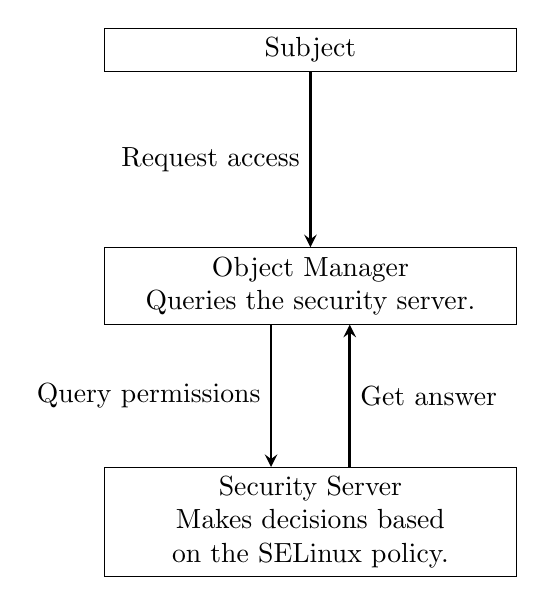
\begin{tikzpicture}
        \usetikzlibrary{calc}
        \tikzstyle{line} = [->,>=stealth, line width=1pt]
        \tikzstyle{rec} = [rectangle, draw=black, align=center, text width=5cm]

        \node(subject) [rec] {Subject};
        \node(objman) [rec, below of=subject, node distance=3cm] {Object
        Manager\\ Queries the security server.};
        \node(secser) [rec, below of=objman, node distance=3cm] {Security
        Server\\ Makes decisions based on the SELinux policy.};

        \draw[line] (subject) -- node[midway,left] {Request access} (objman);
        \draw[line] ([xshift=-0.5cm]objman.south) -- node[midway,left] {Query
        permissions} ([xshift=-0.5cm]secser.north);
        \draw[line] ([xshift=0.5cm]secser.north) -- node[midway,right] {Get
        answer} ([xshift=0.5cm]objman.south);
    \end{tikzpicture}
    \caption{High-level process of policy enforcing}
\end{figure}

For example, when process \texttt{httpd} wants to open the
\texttt{/etc/httpd/conf/httpd.conf} file, the operation is allowed. It is
desirable to allow \texttt{httpd} access its configuration files, so the SELinux
policy contains rules that allow this operation. But if process \texttt{httpd}
would want to write to the \texttt{/etc/passwd} file, the operation would be
denied. Process \texttt{httpd} should not change the \texttt{/etc/passwd} file,
so the rules which would allow this operation are not present in policy.

\subsection{SELinux Components}
% TODO
Figure 2: SELinux components

SELinux \emph{security server} is embedded in the kernel and it obtains the
security policy via userspace tools.

\emph{Object managers} resides mainly in kernel and make use of hooks provided
by Linux Security Module framework. There are object managers for kernel
services such as files, sockets, IPC etc. Userspace object managers are known as
``SELinux-aware'' applications and adds MAC support for X-Windows, D-bus
messaging, databases, etc.

SELinux \emph{security policy} is contained in \texttt{/etc/selinux} directory.
It consists of base policy and several policy modules. Base policy contains
information required by other modules. Policy modules usually supports one
particular service or application (e.g. policy module for Apache web server)
\cite[pp.~20--22]{tsn}.

Maintaining SELinux requires several userspace tools. The \texttt{checkmodule},
\texttt{checkpolicy}, \texttt{load\_policy} commands compile and load policy.
The \texttt{semanage} and \texttt{restorecon} command manages security labels of
various system resources \cite[p.~389]{tsn}.


\section{Mandatory Access Control}
% 2.3 MANDATORY ACCESS CONTROL (MAC)                                    Y

TODO

\subsection{Discretionary Access Control}
Discretionary access control is defined by TCSES standard. System with DAC must
enable users to protect their data by controlling access to that data, e.g. by
setting permissions for other users or user groups.

In DAC, users make security decisions by specifying who can access their data.
The problem is that users can easily propagate information.

Linux implements discretionary access control. Every object has an owner that
controls access to that object. Permissions are set in three scopes: user,
group, and others. For each scope, permissions to read, write and execute can be
set.

\subsection{Mandatory Access Control}
Mandatory access control (MAC), defined by \emph{Trusted Computer System
Evaluation Criteria} (TCSEC) standard \cite{orangebook}, provides more
restrictions than DAC. In this type of access control, operating system can
prevent subjects to perform operations on objects. This is achieved by attaching
subjects and objects set of security attributes. When a subject (usually a
process) wants to perform an operation on an object (file, directory, socket,
etc.), operating system first examines these attributes. Security policy is then
used to determine whether this operation should be allowed or not. When using
MAC, users do not have the ability to override the security policy and, for
example, propagate sensitive information.

There are several implementations of MAC. Linux kernel currently contains
several security modules implemented using \emph{Linux Security Modules} (LSM)
framework \cite{lsmusage}. \emph{Security-Enhanced Linux} (SELinux), developed
by National Security Agency and Red Hat \cite{selinuxcontr}, is used in Red Hat
Enterprise Linux (RHEL), CentOS, Fedora and Android
\cite{selinuxguide,selinuxguidefedora,selinuxandroid}. \emph{AppArmor},
developed by SUSE, is used in SUSE Linux Enterprise, openSUSE and Ubuntu
\cite{apparmor,apparmorubuntu}. There are two other security modules,
\emph{Smack} and \emph{TOMOYO Linux}.

\subsection{SELinux and MAC}
SELinux supports two types of mandatory access control:
\begin{description}
    \item [Type Enforcement] Subjects and objects have a type identifier
        associated which is used to enforce policy rules.
    % TODO cite BLP
    \item [Multi-Level Security (MLS)] It is based on the Bell-La Padula model
        and used when different levels of access are required. There is a
        variant called Multi-Category (MCS). MLS and MCS is used to separate
        applications, for example to prevent two virtual machines from accessing
        each other's files.
\end{description}

\section{TODO: TYPE ENFORCEMENT}
% 2.6 TYPE ENFORCEMENT (TE)                                             Y
    % 2.6.1 Constraints                                                 ?
    % 2.6.2 Bounds                                                      N

TODO - drop this chapter?

\section{SELinux Security Context}
% 2.7 SECURITY CONTEXT                                                  Y

Security decisions are made based on a \emph{security context} which must be
assigned to every subject and object. The security context is sometimes reffered
to as \emph{security label} or just \emph{label}. The security context is a
string in the following form:
\begin{lstlisting}
user:role:type[:range]
\end{lstlisting}
Where:
\begin{description}
    \item [\texttt{user}] The SELinux user.
    \item [\texttt{role}] The SELinux role.
    \item [\texttt{type}] Used by type enforcement.
    \item [\texttt{range}] Used by MLS or MCS. It is optional.
\end{description}

Example of subject security contexts:
\begin{lstlisting}
$ ps -eZ
LABEL                             PID TTY          TIME CMD
system_u:system_r:init_t:s0         1 ?        00:00:04 systemd
system_u:system_r:kernel_t:s0       2 ?        00:00:00 kthreadd
system_u:system_r:auditd_t:s0    1139 ?        00:00:00 auditd
system_u:system_r:alsa_t:s0      1164 ?        00:00:00 alsactl
...
\end{lstlisting}

Example of object security contexts:
\begin{lstlisting}
$ ls -Z /etc
               system_u:object_r:etc_t:s0 alsa
         system_u:object_r:cupsd_etc_t:s0 cups
          system_u:object_r:dhcp_etc_t:s0 dhcp
       system_u:object_r:passwd_file_t:s0 passwd
          system_u:object_r:net_conf_t:s0 resolv.conf
...
\end{lstlisting}

\section{Subjects and Objects}
% 2.8 SUBJECTS                                                          Y
% 2.9 OBJECTS                                                           Y
    % 2.9.1 Object Classes and Permissions                              Y
    % 2.9.2 Allowing a Process Access to Resources                      Y
    % 2.9.3 Labeling Objects                                            Y
        % 2.9.3.1 Labeling Extended Attribute Filesystems               Y
            % 2.9.3.1.1 Copying and Moving Files                        Y
        % 2.9.3.2 Labeling Subjects                                     Y
    % 2.9.4 Object Reuse                                                N

A \emph{subject} is an entity that causes information to flow among objects or
changes the system state. Within SELinux, a subject is an active process that
can access objects. Note that a process can also be an object, for example when
sending signal to another process, the receiving process is an object.

An \emph{object} is a system resource such as file, socket, pipe, TCP or UDP
port, network interface, semaphore or shared memory segment. Objects are
accessed via subjects. Objects are divided into classes based on permission
sets.

\subsection{Object Classes}
% TODO cite reference policy
Each object is assigned class identifier which specifies set of permissions that
describe what operations can object handle. For example, in Reference Policy
version 2.20180114, class \texttt{shm} provides the following permissions:
\begin{lstlisting}
create, destroy, getattr, setattr, read, write, associate, unix_read,
unix_write, lock
\end{lstlisting}
SELinux object classes maps to the kernel object classes (files, sockets, etc.)
and userspace objects (for X-Windows or D-Bus).

\subsection{Allowing a Subject to Access an Object}
Subjects are given access to objects via \texttt{allow} rules in the security
policy. Example of an \texttt{allow} rule:
\begin{lstlisting}
allow httpd_t samba_share_t:file { getattr open read };
\end{lstlisting}
Here the process running with context \texttt{httpd\_t} (Apache HTTP Server) is
given access to file labeled as \texttt{samba\_share\_t} (files shared via
Samba). The allowed operations are \texttt{getattr}, \texttt{open}, and
\texttt{read}. This means that the process can open and read from these files
but it cannot modify them.

\section{Labeling Subjects and Objects}
% 2.10 COMPUTING SECURITY CONTEXTS                                      Y
    % 2.10.1 Security Context Computation for Kernel Objects            Y
        % 2.10.1.1 Process                                              Y
        % 2.10.1.2 Files                                                Y
        % 2.10.1.3 File Descriptors                                     N
        % 2.10.1.4 Filesystems                                          N
        % 2.10.1.5 Network File System (nfsv4)                          N
        % 2.10.1.6 INET Sockets                                         N
        % 2.10.1.7 IPC                                                  N
        % 2.10.1.8 Message Queues                                       N
        % 2.10.1.9 Semaphores                                           N
        % 2.10.1.10 Shared Memory                                       N
        % 2.10.1.11 Keys                                                N
    % 2.10.2 Using libselinux Functions                                 N
        % 2.10.2.1 avc_compute_create and security_compute_create       N
        % 2.10.2.2 avc_compute_member and security_compute_member       N
        % 2.10.2.3 security_compute_relabel                             N

% TODO
Security contexts are computed by the kernel security server using several
policy statements.

\subsection{Labeling Processes}
The first init process usually transitions to its own unique process, for
example \texttt{init\_t}. On fork, a process inherits the security context of
its parent. On exec, a process may transition to different security context.
This is achieved by various transition policy statements. SELinux-aware
processes may change context by calling \texttt{setcon} or \texttt{setexeccon}.

\subsection{Labeling Files}
Security context for files is computed as follows:
\begin{description}
    \item [\texttt{user}] User is inherited from the creating process.
    \item [\texttt{role}] Role defaults to \texttt{object\_r} unless modified by
        \texttt{role\_transition} statement.
    \item [\texttt{type}] Type defaults to the type of the parent directory
        unless modified by \texttt{type\_transition} statement.
    \item [\texttt{range}/\texttt{level}] Defaults to the low/current level of
        the creating process unless modified by \texttt{range\_transition}
        statement.
\end{description}

\section{Type Transitions}
% 2.12 DOMAIN AND OBJECT TRANSITIONS                                    Y
    % 2.12.1 Domain Transition                                          Y
        % 2.12.1.1 Type Enforcement Rules                               Y
    % 2.12.2 Object Transition                                          Y

% TODO explain domain
To run different processes in different domains, we need a way how to
\emph{transition} a process from one domain to another. To attach file a label
different than its parent's label, we need to transition an object from one type
to another. Both can be achieved using the \texttt{type\_transition} statement.

\subsection{Domain Transition}

Starting new process with different security context is called domain
transition. For example, \texttt{systemd} running as \texttt{init\_t} needs to
start the Apache HTTP Server as \texttt{httpd\_t}. Apache executables are
labeled \texttt{httpd\_exec\_t}. The following policy rule allows the
transition:
\begin{lstlisting}
type_transition init_t httpd_exec_t:process httpd_t;
\end{lstlisting}

\subsection{Object Transition}

\section{TODO: MLS AND MCS}
% 2.13 MULTI-LEVEL SECURITY AND MULTI-CATEGORY SECURITY                 Y
    % 2.13.1 Security Levels                                            N
        % 2.13.1.1 MLS / MCS Range Format                               N
        % 2.13.1.2 Translating Levels                                   N
    % 2.13.2 Managing Security Levels via Dominance Rules               N
    % 2.13.3 MLS Labeled Network and Database Support                   N
    % 2.13.4 Common Criteria Certification                              N

TODO

\section{SELinux Modes of Operation}
% 2.15 SELINUX PERMISSIVE AND ENFORCING MODES                           Y

SELinux has three modes of operation. The default mode is \emph{enforcing}. In
this mode, everything which is not allowed by the policy is denied. When a
process tries to perform an action which is not allowed by the policy, it is
logged. In \emph{permissive} mode, SELinux is not enforcing the policy, it only
logs actions. In \emph{disabled} mode, SELinux is turned off.

\section{TODO: LSM AND SELINUX}
% 2.19 LINUX SECURITY MODULE AND SELINUX                                Y
    % 2.19.1 The LSM Module                                             Y
    % 2.19.2 The SELinux Module                                         Y
    % 2.19.2.1 Fork System Call Walk-thorough                           N
    % 2.19.2.2 Process Transition Walk-thorough                         N
    % 2.19.2.3 SELinux Filesystem                                       N

TODO

% other:
% 2.4 SELINUX USERS                                                     ?
% 2.5 ROLE-BASED ACCESS CONTROL (RBAC)                                  ?
% 2.11 COMPUTING ACCESS DECISIONS                                       ?
% 2.14 TYPES OF SELINUX POLICY                                          Y
    % 2.14.1 Example Policy                                             N
    % 2.14.2 Reference Policy                                           Y
    % 2.14.3 Policy Functionality Based on Name or Type                 Y
    % 2.14.4 Custom Policy                                              N
    % 2.14.5 Monolithic Policy                                          Y
    % 2.14.6 Loadable Module Policy                                     Y
        % 2.14.6.1 Optional Policy                                      N
    % 2.14.7 Conditional Policy                                         ?
    % 2.14.8 Binary Policy                                              Y
    % 2.14.9 Policy Versions                                            Y
% 2.17 POLYINSTANTIATION SUPPORT                                        N
    % 2.17.1 Polyinstantiated Objects                                   N
    % 2.17.2 Polyinstantiation support in PAM                           N
        % 2.17.2.1 namespace.conf Configuration File                    N
        % 2.17.2.2 Example Configurations                               N
    % 2.17.3 Polyinstantiation support in X-Windows                     N
    % 2.17.4 Polyinstantiation support in the Reference Policy          N
% 2.18 PAM LOGIN PROCESS                                                N
% 2.20 LIBSELINUX LIBRARY                                               N
% 2.21 SELINUX NETWORKING SUPPORT                                       N
    % 2.21.1 SECMARK                                                    N
    % 2.21.2 NetLabel - Fallback Peer Labeling                          N
    % 2.21.3 NetLabel - CIPSO                                           N
    % 2.21.4 Labeled IPSec                                              N
    % 2.21.4.1 Configuration Examples                                   N

\section{SELinux Policy Language}
Security decisions made by the security server in kernel are resolved using
SELinux policy. The policy is either monolithic (compiled from single source
file) or modular. Modular policy, which is used in Fedora and RHEL, consists of
mandatory base policy source file and loadable modules. In Fedora, almost every
module contains policy for one application or service, such as the
\texttt{apache} or \texttt{xserver} modules.

SELinux policy statements starts with a statement keyword usually followed by
several identifiers and semicolon at the end. Comments starts with a ``\#''.
Example of an allow rule:

\begin{lstlisting}
# This is an allow rule
allow httpd_t httpd_exec_t: file { ioctl read getattr lock map execute open };
\end{lstlisting}

SELinux assigns context to objects in the system. A \emph{SELinux context}
consists of user, role and type. In order to assign objects types, they must be
declared using the type statement.

\begin{lstlisting}
# declare type bin_t
type bin_t;
\end{lstlisting}

For assigning context to a file, the \texttt{file\_contexts} file (which is
compiled together with the policy source file) is used. For assigning contexts
to other objects, there are several policy statements, such as \texttt{portcon}
(for TCP/IP ports), \texttt{nodecon} (for IP addresses), or \texttt{netifcon}
(for network interfaces).

TODO processes, transitions

\section{Problems with SELinux}
TODO

\section{Linux Audit System}
The \emph{Linux Audit system} provides an auditing system for tracking
security-relevant system events. It is used to track file access, monitor system
calls, record commands run by user, record failed login attempts and others
\cite{secguide}. The Linux Audit system does not provide additional security by
itself, it can be only used to discover security violations.

The Linux Audit system consists of kernel and userspace part. Kernel filters
events and sends them to the \emph{audit daemon}. Audit daemon then writes the
received events to log file. There are several userspace tools used for
interacting with the audit system and for working with the log file.

\section{Audit and SELinux}
% 2.16 AUDITING SELINUX EVENTS                                          Y
    % 2.16.1 AVC Audit Events                                           Y
    % 2.16.2 General SELinux Audit Events                               Y

In Fedora and RHEL, SELinux uses the Linux Audit system to log security events.
When a process tries to perform operation without the permissions, an
\emph{Access Vector Cache} (AVC) denial message is logged using the audit daemon
\cite{selinuxguide}. This message can be then processed by tools such as
\texttt{setroubleshoot} or \texttt{audit2allow}.

Every AVC message contains information about \emph{source context} (the context
of the process), \emph{object class} (for example file), and \emph{target
context} (the context of the object). For example, when a process \texttt{httpd}
running in context \texttt{unconfined\_u:system\_r:httpd\_t:s0} is trying to
perform the \texttt{getattr} operation on file \texttt{/var/www/html/file1} with
context \texttt{system\_u:object\_r:samba\_share\_t:s0} and fails, the following
AVC message is generated:

\begin{lstlisting}
type=AVC msg=audit(1223024155.684:49): avc:  denied  { getattr }
for pid=2000 comm="httpd" path="/var/www/html/file1" dev=dm-0
ino=399185 scontext=unconfined_u:system_r:httpd_t:s0
tcontext=system_u:object_r:samba_share_t:s0 tclass=file
\end{lstlisting}

\section{The audit2allow Tool}
The \emph{audit2allow} is a userspace tool that scans the AVC messages and
generates SELinux policy snippets based on them.

\subsection{Purpose of audit2allow}
The audit2allow tool is designed to help administrators troubleshoot SELinux
denials.

TODO: basic mode - generating rules, admin can decide whether they could be
allowed, for development - devels can use permissive domain, run tests, collect
AVC, create basis for policy module, additional useful info - booleans,
interfaces, ...

\subsection{TODO: What It Does}
In default mode, it scans the AVC denial messages and generates policy rules
which allows the operations that were denied.

For example, when the \texttt{httpd} process tries to perform \texttt{getattr}
action on the \texttt{/var/www/html/file1} file, the following AVC message is
generated:
\begin{lstlisting}
type=AVC msg=audit(1223024155.684:49): avc:  denied  { getattr }
for pid=2000 comm="httpd" path="/var/www/html/file1" dev=dm-0
ino=399185 scontext=unconfined_u:system_r:httpd_t:s0
tcontext=system_u:object_r:samba_share_t:s0 tclass=file
\end{lstlisting}
The audit2allow would generate the following policy rule:
\begin{lstlisting}
allow httpd_t samba_share_t:file getattr;
\end{lstlisting}

The audit2allow is able to read AVC messages from stdin, dmesg, audit log, or
arbitrary file. There is \texttt{-{}-boot} option which loads only messages
generated since last boot and \texttt{-{}-lastreload} option which loads only
messages since last policy reload.

The audit2allow can output the policy rules directly to stdout or file, or
create a policy module which can be loaded directly into the policy.

% TODO make sure that booleans are explained earlier
The audit2allow is using currently loaded policy (or any other policy specified
in the \texttt{-{}-policy} option) to get more information about the denials.
For example, audit2allow suggests turning on a boolean that would allow the
denied operations.

When run with the \texttt{-{}-reference} option, audit2allow tries to match the
denials against defined interfaces. Example of audit2allow output without the
\texttt{-{}-reference} option:
\begin{lstlisting}
#============= httpd_t ==============
allow httpd_t samba_share_t:file getattr;
\end{lstlisting}
Example of audit2allow output with the \texttt{-{}-reference} option:
\begin{lstlisting}
require {
	type httpd_t;
}

#============= httpd_t ==============
samba_read_share_files(httpd_t)
\end{lstlisting}
The audit2allow found an interface which contained the same allow
rule. Interfaces creates more readable code but can contain more rules that are
necessary.

TODO: dontaudit rules

\subsection{TODO: How Does audit2allow Work}
The audit2allow first collects audit messages from various sources and then
filters out AVC messages and other useful messages. From every AVC message,
source context, target context, object class, and permissions are extracted and
converted into \emph{access vector sets}. Each access vector has unique source
context, target context, and object class combination. Permissions from multiple
AVC messages are merged into one access vector. Example of an access vector set:
% TODO: do it better
\begin{lstlisting}
{
    ('unconfined_u:system_r:httpd_t:s0',
     'system_u:object_r:samba_share_t:s0',
     'file'): [ 'getattr', 'open' ],
    ('unconfined_u:system_r:httpd_t:s0',
     'system_u:object_r:sssd_conf_t:s0',
     'file'): [ 'getattr' ],
}
\end{lstlisting}

Each access vector is then converted into an allow rule. Example:
\begin{lstlisting}
allow httpd_t samba_share_t:file { getattr, open };
allow httpd_t sssd_conf_t:file getattr;
\end{lstlisting}

Various other information is stored during processing. The audit2allow prints
comments with helpful messages. TODO

\subsection{Implementation of audit2allow}
The audit2allow utility is written mostly in Python with several parts written
in C.  Main script, \texttt{audit2allow}, parses command-line options, retrieves
audit messages, and prints the output.  Main logic of converting AVC denial
messages to access vector rules is implemented in package \texttt{sepolgen}.

The \texttt{sepolgen} package contains the following modules:
\begin{description}
    \item [\texttt{audit}] Defines classes for various audit messages, contains
        audit message parser.
    \item [\texttt{access}] Defines access vectors and access vector sets.
    \item [\texttt{policygen}] Creates policy rules based on access vectors.
    \item [\texttt{refpolicy}] Contains classes that represent the policy
        statements.
    \item [\texttt{output}] Outputs the generated rules.
    \item [Other modules] There are several other modules which are either not
        significant (e.g. the \texttt{utils} package) or used only for
        generating policy using interfaces (e.g. the \texttt{interfaces}
        package).
\end{description}

\subsubsection{The audit2allow Script}
% parse options
% load policy
    % init the audit2why C module
% read input
    % creates audit parser
    % reads messages
    % feeds them to the parser
% process input
    % filters messages if neccessary
    % converts messages to access vectors
% output
    % output audit2why if selected
    % creates policy generator
    % sets options to the generator
    % adds AVs to the generator
    % writes the output

The main script does the following steps:
\begin{enumerate}
    \item Parse command-line arguments and check potential conflicts.
    \item Read audit messages. Create \texttt{AuditParser} instance and feed it
        the messages.
    \item Filter the messages (if specified by the \texttt{-{}-type} option) and
        convert them to access vectors.
    \item Create and setup a \texttt{PolicyGenerator} instance, feed it the
        access vectors, and convert them to policy rules.
    \item Write the output.
\end{enumerate}

\subsubsection{The audit Module}
% convenience functions
% AuditMessage class
    % base class for all messages
% InvalidMessage class
% PathMessage class
% PolicyLoadMessage class
% DaemonStartMessage class
% ComputeSidMessage class
% AVCMessage class
    % from_split_string
    % analyze
% AuditParser class
    % parse_file, parse_string
    % to_role, to_access
% AVCTypeFilter
% ComputeSidTypeFilter

The \texttt{audit} module is used for parsing audit messages. The
\texttt{AuditParser} class reads strings and creates objects of appropriate type
for each message. The \texttt{AuditMessage} class is the base class for all
message types. The \texttt{AVCMessage} class represents AVC denials and is used
for generating access vectors.

After parsing of AVC message, the denial is analyzed in \texttt{audit2why}
module. The \texttt{audit2why} module tries to find out the reason of the denial
by analyzing the policy. The module is written in C and uses the
\texttt{libsepol} library. Each message is then converted to an access vector
from the \texttt{access} module.

\subsubsection{The access Module}
% AccessVector
    % basic representation of access
    % single source and target type, single object class, set of permissions
% AccessVectorSet
    % used for storing AVs
    % AVs with same source and target type and class are merged
    % add() adds AV to the set
% RoleTypeSet

The \texttt{access} module defines the \texttt{AccessVector} and
\texttt{AccessVectorSet} classes. Access vector is a basic representation of an
access in SELinux. It contains single source and target type, single object
class, and set of permissions. Every AVC denial message can be converted into an
access vector. For example this AVC denial message:
\begin{lstlisting}
type=AVC msg=audit(1223024155.684:49): avc:  denied  { getattr }
for pid=2000 comm="httpd" path="/var/www/html/file1" dev=dm-0
ino=399185 scontext=unconfined_u:system_r:httpd_t:s0
tcontext=system_u:object_r:samba_share_t:s0 tclass=file
\end{lstlisting}
would be converted into the following access vector:
\begin{lstlisting}
{
    source_context: 'unconfined_u:system_r:httpd_t:s0',
    target_context: 'system_u:object_r:samba_share_t:s0',
    object_class: 'file',
    permissions: [ 'getattr' ]
}
\end{lstlisting}

Multiple access vectors are aggregated in access vector sets. Access vectors
that share the same source and target type and object class are merged together
so that there are no duplicates. Access vector sets serves as a basis for
generating policy access vector rules in \texttt{policygen} module.

\subsubsection{The policygen Module}
% PolicyGenerator
    % generates policy module from access vectors
    % has several options
    % set_gen_refpol()
    % set_gen_requires()
    % set_gen_explain()
    % set_gen_dontaudit()
    % add_access()
% explain_access()
% call_interface()
% InterfaceGenerator
% gen_requires()

The \texttt{policygen} module defines \texttt{PolicyGenerator} class that
generates policy module from access vectors. The \texttt{PolicyGenerator}
converts access vector set into SELinux policy statements. For example, this
access vector:
\begin{lstlisting}
{
    source_context: 'unconfined_u:system_r:httpd_t:s0',
    target_context: 'system_u:object_r:samba_share_t:s0',
    object_class: 'file',
    permissions: [ 'getattr', 'open', 'read' ]
}
\end{lstlisting}
would be converted into this policy statement:
\begin{lstlisting}
allow httpd_t samba_share_t:file { getattr open read };
\end{lstlisting}

The \texttt{PolicyGenerator} uses objects from the \texttt{refpolicy} module to
represent policy statements. The \texttt{PolicyGenerator} provides several
configuration methods:
\begin{description}
    \item [\texttt{set\_gen\_refpol()}] Turn on interface generation.
    \item [\texttt{set\_gen\_requires()}] Add module requires (neccessary for
        creating a standalone policy module).
    \item [\texttt{set\_gen\_explain()}] Add comments explaining why were the
        policy statements generated.
    % TODO: make sure that dontaudit rules are explained earlier
    \item [\texttt{set\_gen\_dontaudit()}] Generate \texttt{dontaudit} rules
        instead of \texttt{allow} rules.
\end{description}
The output of the \texttt{PolicyGenerator} is a tree-like structure containing
generated statements. The \texttt{output} module then just prints out every
statement.

\chapter{Analysis}
Several improvements to audit2allow were proposed:
\begin{enumerate}
    \item Changing label of an object instead of creating new policy rules. This
        includes checking of mislabeled files, labeling network ports, nodes,
        and interfaces.
    \item Support for new SELinux policy statements.
\end{enumerate}

\section{Mislabeled Files}
SELinux relies on files that are correctly labeled. Sometimes, files get
mislabeled and causes AVC denials. When used for troubleshooting, audit2allow
suggests adding new rules to the policy instead of changing label of the file.

\subsection{Labeling of Files}
When accessing files, SELinux relies on labels stored with those files to make a
security decision. SELinux labels can be viewed using the \texttt{ls -Z}
command:
\begin{lstlisting}
$ ls -Z
unconfined_u:object_r:user_home_t:s0    testdir
unconfined_u:object_r:user_home_t:s0    testfile
\end{lstlisting}
Labels are stored in extended attributes in the security namespace
\cite{xattrman}:
\begin{lstlisting}
$ getfattr -n security.selinux testfile
# file: testfile
security.selinux="unconfined_u:object_r:user_home_t:s0"
\end{lstlisting}

There are rules in policy that specifies the context of files created by
processes. For example, when process running with \texttt{httpd\_t} context
creates a file in directory with \texttt{var\_run\_t} context, the file will get
context \texttt{httpd\_var\_run\_t}:
% TODO explain
\begin{lstlisting}
$ sesearch -T -s httpd_t -t var_run_t -c file
type_transition httpd_t var_run_t:file httpd_var_run_t;
\end{lstlisting}

There are situations when files get label that is different than the default
one:
\begin{enumerate}
    % TODO fix
    \item When moving files, label is preserved. This does not happen when
        copying files because new file is always created.
    \item When SELinux is disabled, labels are not assigned to files.
    \item When policy is changed (for example when a module is unloaded), there
        may be some files left with type that is no longer defined in policy.
\end{enumerate}
For these situations, there is a \texttt{file\_contexts} file which specifies
default contexts for every file. Example:
\begin{lstlisting}
/run/.*         --  system_u:object_r:var_run_t:s0
/var/.*	        --  system_u:object_r:var_t:s0
/etc/.*	        --  system_u:object_r:etc_t:s0
/lib/.*	        --  system_u:object_r:lib_t:s0
/usr/.*\.cgi    --  system_u:object_r:httpd_sys_script_exec_t:s0
/root(/.*)?     --  system_u:object_r:admin_home_t:s0
/dev/[0-9].*    -c  system_u:object_r:usb_device_t:s0
/dev/.*tty[^/]* -c  system_u:object_r:tty_device_t:s0
\end{lstlisting}
The \texttt{-{}-} is means every file type, \texttt{-c} means character device.
The \texttt{restorecon} utility is used to restore security contexts on files.

\subsection{AVC Denial Messages Caused by Mislabeled Files}
When a process is trying to access file that is mislabeled, the operation is
usually denied (unless the process has access also to the new label). Similar
AVC denial message is generated:
\begin{lstlisting}
type=AVC msg=audit(1226270358.848:238): avc:  denied  { getattr }
for  pid=13349 comm="httpd" path="/var/www/html/index.html"
dev=dm-0 ino=218171 scontext=system_u:system_r:httpd_t:s0
tcontext=system_u:object_r:user_home_t:s0 tclass=file
\end{lstlisting}
File \texttt{/var/www/html/index.html} is mislabeled, because files in
\texttt{/var/www/html} should have context \texttt{httpd\_sys\_content\_t}. This
denial should be fixed by running \texttt{restorecon} on the file:
\begin{lstlisting}
# restorecon -v /var/www/html/index.html
Relabeled /var/www/html/index.html from unconfined_u:object_r:user_home_t:s0
to unconfined_u:object_r:httpd_sys_content_t:s0
\end{lstlisting}

When using audit2allow, the following rules are generated:
\begin{lstlisting}
allow httpd_t user_home_t:file getattr;
\end{lstlisting}
This solution is not secure because it is adding unnecessary rules to the policy
and it does not solve the real problem.

\subsection{Proposal for Improvement to audit2allow}
The audit2allow should detect when the AVC message is caused by mislabeled file
and suggest solution using the \texttt{restorecon} utility.

There are three fields in the AVC message that can be used to detect if the file
was mislabeled: \texttt{path}, \texttt{name} and \texttt{inode}. When the
\texttt{path} field is present, audit2allow can run \texttt{matchpathcon} to get
the default context of the file and compare it with actual file context.

In many cases, the \texttt{path} field is not present, only inode number and
name of the file (without full path). In this case it is difficult to find the
full path of the file. Ryan Hallisey created solution \cite{restoreconpullreq}
that is using \texttt{locate} utility to get all files matching the name and
then stat these files to get the inode number. This solution is only partial, it
does not work on files that are not indexed in the database created by
\texttt{updatedb}.

\section{Extended Permission Access Vector Rules}
Since policy version 30, there are extended permission access vector (AV) rules
that expand the permission sets. Access vector rules operates with 32~bit
permission sets, extended permission AV rules adds arbitrary number of 256~bit
increments. Extended permission AV rules are currently (policy version 31) used
only for ioctl whitelisting, but they provide generic tool that can be used in
future for more granular control over an operation \cite{selinuxmailxperms}.

\subsection{Syntax and Usage of Extended Permission AV Rules}
The format of extended permission AV rules is \cite{xpermrules}:
\begin{lstlisting}
rule_name source_type target_type : class operation xperm_set;
\end{lstlisting}
where:
\begin{description}
    \item [\texttt{rule\_name}] is one of the following: \texttt{allowxperm},
        \texttt{dontauditxperm}, \texttt{auditallowxperm}, or
        \texttt{neverallowxperm}. The meaning is similar to standard AV rules.
    \item [\texttt{source\_type}, \texttt{target\_type}, \texttt{class}] are
        source type, target type, and object class, same as with standard AV
        rule.
    \item [\texttt{operation}] is a single keyword defining the operation to be
        implemented by the rule. As of policy version 31, only \texttt{ioctl}
        operation is supported.
    \item [\texttt{xperm\_set}] are extended permissions represented by numeric
        values.
\end{description}

Example of an extended permission AV rule:
\begin{lstlisting}
allowxperm my_app_t my_socket_t : tcp_socket ioctl { 20 30 0x40 50-60 };
\end{lstlisting}

Process running as \texttt{my\_app\_t} can call ioctl on a TCP socket labeled
\texttt{my\_socket\_t} with parameters 20, 30, 64, or any number from 50 to 60.

In order for ioctl whitelisting to work, standard \texttt{allow} rule must be
present in the policy. With \texttt{allow} rule for ioctl, all ioctl syscalls
are allowed. With additional \texttt{allowxperm} rule, only specified values are
allowed.

\subsection{AVC Denials Caused by Extended Permission AV Rules}
Suppose there are following rules present in the policy:
\begin{lstlisting}
allow src_t tgt_t : tcp_socket ioctl;
allowxperm src_t tgt_t : tcp_socket ioctl 0x42;
\end{lstlisting}
When the process tries to call \texttt{ioctl(0x1234, ...)}, the operation would
be denied, because only syscall \texttt{ioctl(0x42, ...)} is allowed. The
following AVC denial message would be generated:
\begin{lstlisting}
type=AVC msg=audit(1515017775.689:1722): avc:  denied  { ioctl } for
pid=14587 comm="test" dev="dm-0" ino=8390105 ioctlcmd=0x1234
scontext=unconfined_u:unconfined_r:src_t:s0-s0:c0.c1023
tcontext=unconfined_u:object_r:tgt_t:s0 tclass=tcp_socket permissive=0
\end{lstlisting}
Field \texttt{ioctlcmd} contains first parameter of ioctl syscall that was
denied. This value can be used to construct an allowxperm rule to allow this
operation.

When used for troubleshooting this AVC denial, audit2allow produces the
following output:
\begin{lstlisting}
#============= src_t ==============

#!!!! This avc is allowed in the current policy
allow src_t tgt_t:tcp_socket ioctl;
\end{lstlisting}
which is not helpful. Administrator must know about extended permissions and
assume that the allow rule was overridden.

\subsection{Generating Extended permission AV rules in audit2allow}
The audit2allow does have all the information to generate extended permission AV
rules. First of all, it should warn user, that the operation may have been
denied because of extended permission AV rules. In the preceding example, there
should be a warning message. Then there should be a way how to generate extended
permission AV rules from AVC messages, for example a command-line option.

TODO: discussion about default behaviour.

\section{Labeling Network Ports, Nodes and Interfaces}
SELinux policy supports labeling of TCP and UDP ports, network nodes
(represented by IP addresses and subnet masks), and network interfaces (e.g.
\texttt{eth0}).

\subsection{Network Ports}
SELinux can enforce binding to system ports. For example, in Fedora 27, there
are several hundred \texttt{portcon} rules that label TCP and UDP ports.
Example:
\begin{lstlisting}
$ seinfo --portcon

Portcon: 615
   portcon tcp 1-511 system_u:object_r:reserved_port_t:s0
   portcon tcp 7 system_u:object_r:echo_port_t:s0
   portcon tcp 21 system_u:object_r:ftp_port_t:s0
   portcon tcp 22 system_u:object_r:ssh_port_t:s0
   portcon tcp 53 system_u:object_r:dns_port_t:s0
   portcon tcp 80 system_u:object_r:http_port_t:s0
   portcon udp 1-511 system_u:object_r:reserved_port_t:s0
   portcon udp 1 system_u:object_r:inetd_child_port_t:s0
   portcon udp 7 system_u:object_r:echo_port_t:s0
   portcon udp 53 system_u:object_r:dns_port_t:s0
   portcon udp 67 system_u:object_r:dhcpd_port_t:s0
   ...
\end{lstlisting}
Portcon rules can overlap, for example TCP port number 80 is labeled
\texttt{http\_port\_t} but also \texttt{reserved\_port\_t} because it is in range
1--511. Every port has either domain-specific label or of the following labels
(based on range):

\begin{tabular}{l l}
    1--511 & \texttt{reserved\_port\_t} \\
    512--1023 & \texttt{hi\_reserved\_port\_t} \\
    1024--32767 & \texttt{unreserved\_port\_t} \\
    32768--61000 & \texttt{ephemeral\_port\_t} \\
    61001--65535 & \texttt{unreserved\_port\_t} \\
\end{tabular}

When a process tries to bind port and it is denied by policy, AVC message is
generated. For example:
\begin{lstlisting}
type=AVC msg=audit(1516026512.648:4191): avc:  denied  { name_bind } for
pid=6116 comm="test" src=43 scontext=unconfined_u:unconfined_r:my_app_t:s0
tcontext=system_u:object_r:reserved_port_t:s0
tclass=tcp_socket permissive=0
\end{lstlisting}

Proper way how to allow the process to bind on port number 43 would be to label
this port with a application-specific context. The audit2allow suggest adding
the following rule to the policy:
\begin{lstlisting}
allow my_app_t reserved_port_t:tcp_socket name_bind;
\end{lstlisting}
This rule would allow \texttt{my\_app\_t} access to all reserved ports which is
unneccessary and potentially unsecure.

Ports can be labeled using the \texttt{portcon} rules, but as of policy version
31, these rules are not valid in policy module, only in base policy. So
audit2allow would not be able to generate \texttt{portcon} rules directly.
Another way of labeling ports is via the \texttt{semanage port} command. The
audit2allow should suggest using the \texttt{semanage port} command when
appropriate.

\subsection{Network Nodes}
TODO

\subsection{Network Interfaces}
TODO

\chapter{Implementation}
From the list of possible improvements to audit2allow, extended permissions were
implemented.

\section{Extended permissions}
Modules \texttt{audit}, \texttt{access}, \texttt{policygen}, \texttt{refpolicy}
were modified to support extended permissions. New command-line option
\texttt{-{}-xperms} was added to turn on generating of the extended permission
access vector rules.

\subsection{Parsing AVC Denial Messages}
The \texttt{audit} module was extended to parse \texttt{ioctlcmd} field in AVC
denial messages. The \texttt{ioctlcmd} field is then converted to fit the
general concept of extended permissions and passed to the access vector set.

\subsection{Storing Extended Permissions in Access Vector Sets}
Extended permissions are stored inside an access vector as a dictionary, where
the operation is the key. Example of extended permissions:
\begin{lstlisting}
{
    'ioctl': <refpolicy.XpermSet() object>,
    'other_command': <refpolicy.XpermSet() object>,
    'another_command': <refpolicy.XpermSet() object>,
}
\end{lstlisting}
The \texttt{AccessVectorSet} was modified to correctly merge two access vectors
with extended permissions attached.

\subsection{Representation of Extended Permission AV Rules}
Extended permission access vector rules are represented in the
\texttt{refpolicy} module by the \texttt{AVExtRule} class. These rules are
created from access vectors using the \texttt{from\_av()} method. Method
\texttt{to\_string()} prints out the rule. Example of an extended permission AV
rule:
\begin{lstlisting}
allowxperm my_app_t my_socket_t : tcp_socket ioctl { 20 30 0x40 50-60 };
\end{lstlisting}

The extended permission set (in the previous listing \texttt{\{ 20 30 0x40 50-60
\}}) is represented by separate class \texttt{XpermSet}.

\subsection{Generating Extended Permission AV rules}
Without extended permissions, every access vector can be converted into single
AV rule. With extended permissions attached to the access vector, to fully
convert access vector to policy rules, there needs to be one AV rule and
possibly several extended permission AV rules. For example, this access vector:
% TODO use different contexts and tcp_socket
\begin{lstlisting}
{
    source_context: 'unconfined_u:system_r:httpd_t:s0',
    target_context: 'system_u:object_r:samba_share_t:s0',
    object_class: 'file',
    permissions: [ 'getattr', 'ioctl', 'open' ]
    extended_permissions: {
        'ioctl': [ 1, 2, 3 ],
        'other_command': [ 40, 50, 60 ],
        'another_command': [ 700, 800, 900 ],
    }
}
\end{lstlisting}
would be converted into these policy rules\footnote{Note that as of policy
version 31, only the \texttt{ioctl} operation is supported, operations
\texttt{other\_command} and \texttt{another\_command} were added only as an
example.}:
\begin{lstlisting}
allow httpd_t samba_share_t:file { getattr ioctl open };
allowxperm httpd_t samba_share_t:file ioctl { 1 2 3 };
allowxperm httpd_t samba_share_t:file other_command { 40 50 60 };
allowxperm httpd_t samba_share_t:file another_command { 700 800 900 };
\end{lstlisting}

The \texttt{PolicyGenerator} was modified to generate extended permission AV
rules for every operation in access vector. New configuration method was added,
\texttt{set\_gen\_xperms()}, to specify whether the extended permission AV rules
should be generated.

\chapter{Functional Testing}
TODO: about tests, chosen coverage

\section{Unit Tests}

TODO: test\_access

TODO: test\_audit

TODO: test\_policygen

TODO: test\_refpolicy

\section{Integration Tests}

TODO

\chapter{Summary}
TODO
